\documentclass{article}
\usepackage[utf8]{inputenc}
\usepackage{amsmath}
\usepackage{graphicx}
\usepackage{float}
\usepackage[font=scriptsize,labelfont=bf]{caption}

\title{COMP6245 : Lab 5 Report}
\author{Thanakorn Panyapiang(tp2n19@soton.ac.uk)}
\date{}

\begin{document}
\maketitle

The performance of the original RBF implementation with 200 basis functions is show in Figure 1. The graph indicates that the model is significantly overffited with the training data and perform poorly on the test set.

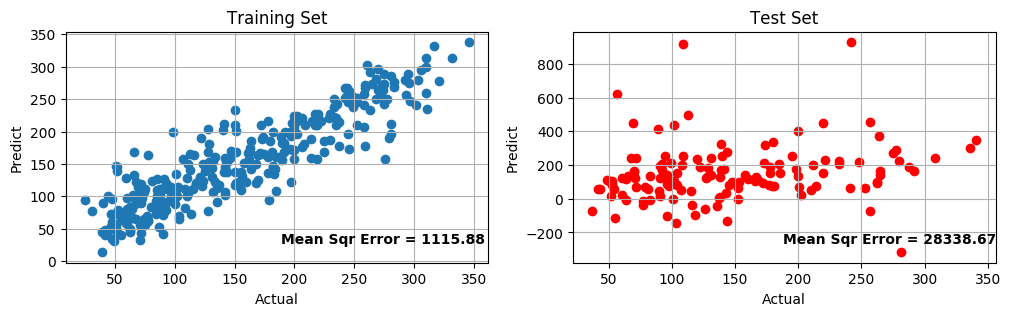
\includegraphics[scale=0.4]{rbf_original}
\captionof{figure}{}

To improve the model, the following changes have been added:
\begin{enumerate}
\item Normalizing each feature so its value is between 0 to 1.
\item Computing the width of basis functions($\sigma$) using average pairwise distance of 50 points which are randomly sampled from the training set.
\item Computing locations of the basis functions using K-mean clustering where K is set to be 30.
\end{enumerate}

\indent After above-mentioned improvements, although the error on the training set increases, the model accuracy on the test set is significantly better than the original version as can be seen from Figure 2. However, if the value of M is set to be very high(f.e. 100), the model is still overfiffed with the training data similar the original implementaion.

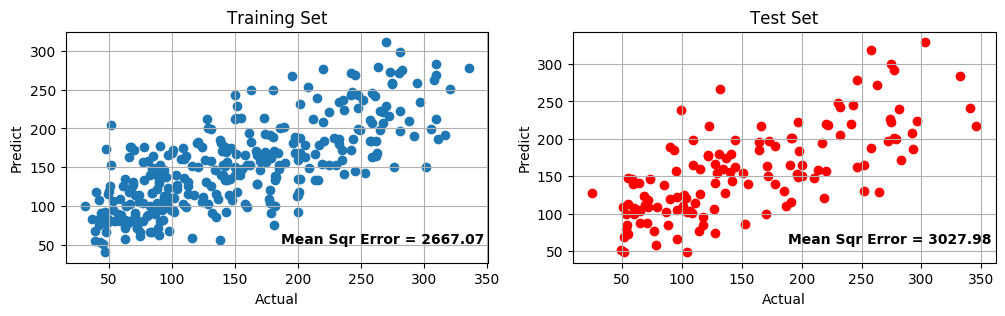
\includegraphics[scale=0.4]{rbf_improved}
\captionof{figure}{}

To compare RBF with Linear Regression(with L2 regularization), the data has been splitted into 10 parts to run ten-fold cross validation. The sample distributions of predicted values of both models are shown in the figure below. One thing which can be noticed is that RBF model generaly has a wider range of predicted values.

\begin{center}
\begin{tabular}{cccc}
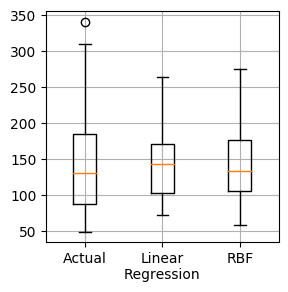
\includegraphics[scale=0.3]{result_dist_1} &
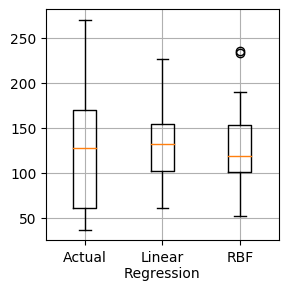
\includegraphics[scale=0.3]{result_dist_2} &
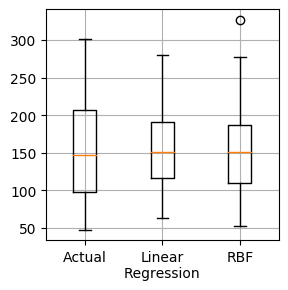
\includegraphics[scale=0.3]{result_dist_3} &
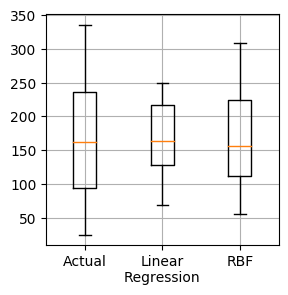
\includegraphics[scale=0.3]{result_dist_4}
\end{tabular}
\captionof{figure}{}
\end{center}

\end{document}